\chapter{Scenarios and use cases}
\label{ch:scenarios}

\section{User related scenarios}
\newcommand{\see}[1][reference missing]{(see \specref{#1})}
The buttons and the yellow border in scenario 1 to 4 are specified in \autoref{ch:sysmodels}, User interface.

\subsection{Scenario 1: User successfully records a session}
\begin{enumerate}
    \item The application shows a button at the bottom right corner of the screen.
    \item \Gls{user} clicks the button to start recording.
    \item The application starts to record and shows a yellow border on screen during the whole recording time to indicate that the \gls{session} is being recorded.
    \item \Gls{user} researches in different databases during recording.
    \item \Gls{user} finishes the research and clicks the same button to stop recording.
    \item The application shows a dialog to ask the \gls{user}, if the recording data should be saved or not.
    \item \Gls{user} clicks "save" to save the recorded data.
    \item The application saves the recorded data and the yellow border disappears at the same time.
\end{enumerate}

\subsection{Scenario 2: User discards a session}
\begin{enumerate}
    \item The application shows a button at the bottom right corner of the screen.
    \item \Gls{user} clicks the button to start recording.
    \item The application starts to record and shows a yellow border on screen during the whole recording time to indicate that the \gls{session} is being recorded.
    \item \Gls{user} is interrupted by multiple received Emails and reads the Emails for a long period of time.
    \item \Gls{user} realizes that the research only takes up 10\% of the total recording time and gives up on recording by clicking the same button.
    \item The application shows a dialog to ask the \gls{user}, if the recording data should be saved or not.
    \item \Gls{user} clicks "discard" to discard the recorded data.
    \item The application discards the recorded data and the yellow border disappears at the same time.
\end{enumerate}

\subsection{Scenario 3: The minimal recording duration is not reached}
Notice: This scenario covers features declared optional.
\begin{enumerate}
    \item The application shows a button  at the bottom right corner of the screen.
    \item \Gls{user} clicks the button to start recording.
    \item The application starts to record and shows a yellow border on screen during the whole recording time to indicate that the \gls{session} is being recorded.
    \item \Gls{user} is immediately interrupted by an Email after the start of recording and decides to stop recording and read the Email first.
    \item \Gls{user} clicks the same button to stop recording.
    \item The application shows a dialog indicating that the minimal recording duration \see[OC10] is not reached and thus the recorded data will be automatically discarded.
    \item \Gls{user} clicks "confirm" button on the dialog and closes it.
    \item The application discards the recorded data and the yellow border disappears at the same time.
    \end{enumerate}
    
\subsection{Scenario 4: The maximal recording duration is reached}
Notice: This scenario covers features declared optional.
\begin{enumerate}
    \item The application shows a button at the bottom right corner of the screen.
    \item \Gls{user} clicks the button to start recording.
    \item The application starts to record and shows a yellow border on screen during the whole recording time to indicate that the \gls{session} is being recorded.
    \item \Gls{user} researches in different databases during recording but leaves their \gls{device} without terminating the recording.
    \item The application shows a dialog, warning that the maximal duration of the recording \gls{session} \see[OC10] is almost reached.
    \item The maximal duration of the recording \gls{session} \see[OC10] is reached. The application shows a dialog to ask the \gls{user}, if the recording data should be saved or not.
    \item \Gls{user} is back and clicks "save" to save the recorded data.
    \item The application saves the recorded data and the yellow frame disappears at the same time.
\end{enumerate}

\section{Scientist related scenarios}
\subsection{Scenario 5: Scientist extracts data}
\begin{enumerate}
    \item \Gls{scientist} starts the command line tool(see \autoref{ch:sysmodels} Data extraction) provided by the application.
    \item \Gls{scientist} types in commands including the path of the data and an output directory to extract the data from that path to the output directory.
    \item \Gls{scientist} can now use the extracted data in the output directory.
\end{enumerate}


\section{Administrator related scenarios}
\subsection{Scenario 6: Administrator changes configuration}
\begin{enumerate}
    \item The \gls{admin} opens the configuration file provided by the application.
    \item The \gls{admin} changes the maximal recording duration \see[OC10] by editing the configuration file and saving it.
    \item The \gls{admin} distributes the changed configuration file to a \gls{user}.
    \item The \gls{user}'s application receives the changed configuration file .
    \item The maximal recording duration \see[OC10] of the application is changed according to the received configuration file.
\end{enumerate}

\section{Use cases}
\begin{center}
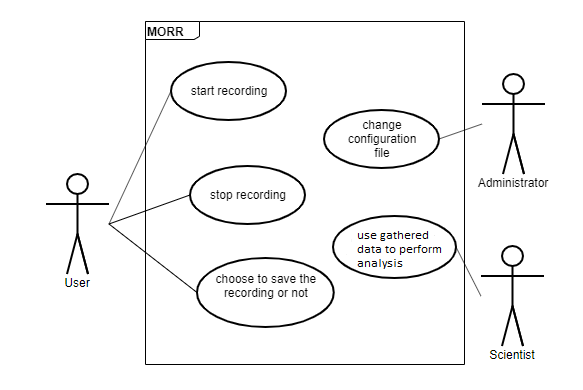
\includegraphics[scale=0.9]{resources/usecase.png}
\end{center}